\documentclass{amsart}
\usepackage{tikz}
\usepackage{booktabs}
\usepackage{hyperref}
\hypersetup{hidelinks}
\theoremstyle{plain}
\newtheorem{theorem}{Theorem}[section]
\newtheorem{lemma}[theorem]{Lemma}
\newtheorem{proposition}[theorem]{Proposition}
\theoremstyle{definition}
\newtheorem{definition}[theorem]{Definition}
\newtheorem{convention}[theorem]{Convention}
\newtheorem{example}[theorem]{Example}
\theoremstyle{remark}
\newtheorem{remark}[theorem]{Remark}

\begin{document}
\title[Two degrees or two face sizes]{No alternating plane graph has exactly two
       vertex degrees, or exactly two face sizes}
\author{Hanyu Yang}
\address{Independent researcher, California, USA}
\email{hanyu.yang.92@gmail.com}
\subjclass[2020]{Primary 05C10; Secondary 05C30}
\keywords{alternating plane graph, plane graph, discharging, Euler's formula}

\begin{abstract}
In an alternating plane graph, adjacent vertices have different degrees and
adjacent faces have different sizes. We prove the conjecture of Alth\"ofer,
Haugland, Scherer, Schneider and Van Cleemput that no such graph has exactly two
degrees, and none has exactly two face sizes. Give every edge the reciprocals of
its two end degrees and its two face sizes. These charges sum to $e+2$. Two
values on one side make the graph bipartite on that side, which forces even
values on the other side, and then no edge gets more than $1$. The result still
holds when bridges are allowed; there a large face on each bridge pays for the
few edges that can exceed $1$.
\end{abstract}

\maketitle

\section{Introduction}

An alternating plane graph is a plane graph in which neighbours differ: adjacent
vertices have different degrees, and adjacent faces have different sizes. How
few degrees and sizes can such a graph get away with? Alth\"ofer, Haugland,
Scherer, Schneider and Van Cleemput~\cite{AHSSV2015}, who introduced these
graphs, conjectured that the answer is three of each:

\begin{quote}
\textbf{Conjecture 10.1.} There are no $2,Y$-alternating plane graphs and no
$X,2$-alternating plane graphs.
\end{quote}

\noindent Here an $X,Y$-alternating plane graph has exactly $X$ distinct degrees
and exactly $Y$ distinct face sizes. Two is the natural first case: alternation
on vertices alone already forces at least two degrees.

They showed that a $2,Y$-alternating plane graph has degrees $3$ and $4$, or
$3$ and $5$, with at least $25$ or $56$ vertices respectively, beyond the reach
of their \texttt{plantri}~\cite{BM2007} search. For weak alternating plane
graphs, which allow degree $2$, they bounded the number of faces by summing
$1/r+1/s$ over edges between an $r$-face and an $s$-face.

That face count never uses degree $2$, and it is most of the proof. Add the same
count over the two ends of each edge. By Euler's formula the four reciprocals,
summed over all edges, give $e+2$, so some edge carries more than $1$.
Alternation alone allows $\frac13+\frac14$ on each side, which is $\frac76$ and
too much. But two values on one side make the graph bipartite there, so the
values on the other side are even. Distinct even values are at least $4$ and
$6$, and $\frac14+\frac16=\frac5{12}$. Now $\frac7{12}+\frac5{12}=1$ at every
edge, a contradiction.

We prove the conjecture in \S\ref{sec:101} (Theorem~\ref{thm:101}). In
\S\ref{sec:c2} we allow bridges, requiring face alternation only between
distinct faces, and show that both statements survive. This is the harder part.

This charge belongs to the tradition of Lebesgue~\cite{Lebesgue1940} and
Kotzig~\cite{Kotzig1955}, now the discharging method~\cite{CW2017, JV2013}.
Here almost nothing is discharged.

\section{Preliminaries}\label{sec:prelim}

All graphs are finite, simple, plane and connected, and faces include the
unbounded one.

\begin{definition}[\cite{AHSSV2015}, Definition~2.1]\label{def:apg}
An \emph{alternating plane graph} is a connected plane graph in which
(a) every vertex has degree at least $3$; (b) every face has size at least $3$;
(c) adjacent vertices have different degrees; (d) adjacent faces have different
sizes. An \emph{$X,Y$-alternating plane graph} is one with exactly $X$ distinct
vertex degrees and exactly $Y$ distinct face sizes.
\end{definition}

\begin{convention}[face size]\label{conv:c1}
The size of a face is the length of its boundary walk~\cite[\S3.3]{MT2001}. A
bridge lies on one face from both sides and counts twice towards its size.
\end{convention}

In a bipartite plane graph every closed walk is even, so every face has even
size under this convention. Counting distinct boundary vertices would lose that.

\begin{convention}[bridges]\label{conv:c2}
In (d), the faces on the two sides of an edge must have different sizes, so a
bridge breaks (d) and alternating plane graphs have none~\cite{AHSSV2015}. A
plane graph is \emph{bridge-relaxed alternating} if it satisfies (a)--(c), and
(d) for distinct adjacent faces.
\end{convention}

\section{The edge charge}\label{sec:identity}

\begin{lemma}\label{lem:identity}
Let $G$ have $v$ vertices, $e \ge 1$ edges and $f$ faces. For an edge $a=uw$
with faces $F^-(a)$ and $F^+(a)$ on its two sides, put
\[
  c(a) \;=\; \frac{1}{\deg u} + \frac{1}{\deg w}
           + \frac{1}{|F^-(a)|} + \frac{1}{|F^+(a)|}.
\]
Then $\sum_a c(a) = v + f = e + 2$. Equivalently the excesses
$x(a) = c(a)-1$ satisfy
\begin{equation}\label{eq:identity}
  \sum_{a} x(a) \;=\; 2 .
\end{equation}
\end{lemma}

\begin{proof}
Each vertex hands $1/\deg$ to each edge end at it, and each face hands $1/|F|$
to each edge side on its boundary walk. Each pays out exactly $1$, so the edges
receive $v+f$, which is $e+2$ by Euler's formula.
\end{proof}

A bridge has $F^-(a)=F^+(a)$ and receives $2/|F|$ from that face. So the lemma
holds with bridges too, and \S\ref{sec:c2} uses it that way.

\begin{example}\label{ex:worked}
Replace each side of a triangle by two paths of length two. This gives $9$
vertices, $12$ edges and $5$ faces. Every edge joins degree $2$ to degree $4$
and separates a quadrilateral from a hexagon, so $c(a)=\frac76$ and the $12$
excesses sum to $2$. Only the degree-$2$ vertices keep it from being
alternating. It also attains the face bound $f \le \frac5{12}e$
of~\cite[(9.5)]{AHSSV2015}.
\end{example}

The second ingredient is parity. At a vertex $u$ of degree $d$, list the edges in
cyclic order $a_1,\dots,a_d$, and call the region between $a_i$ and $a_{i+1}$ a
\emph{corner}. The two corners beside $a_i$ lie in the same face exactly when
$a_i$ is a bridge.

\begin{lemma}[parity]\label{lem:parity}
Suppose the faces of $G$ have a $2$-colouring that is proper on distinct
adjacent faces. Then $\deg u$ minus the number of bridges at $u$ is even, for
every vertex $u$.
\end{lemma}

\begin{proof}
Going once round $u$, the colour changes across each non-bridge edge and stays
the same across each bridge. We return to the first colour, so the number of
changes is even.
\end{proof}

With no bridges, every degree is even. In an $X,2$-alternating graph the two face
sizes give the colouring.

\section{Conjecture 10.1}\label{sec:101}

\begin{theorem}\label{thm:101}
There is no $2,Y$-alternating plane graph and no $X,2$-alternating plane graph.
\end{theorem}

The two cases exchange vertices and faces (Table~\ref{tab:budget}). They are not
formally dual. Duality needs $3$-edge-connectivity~\cite[Lemma~2.2]{AHSSV2015},
since a $2$-edge cut gives parallel edges in the dual. So we prove both.

\begin{table}[ht]
\centering
\begin{tabular}{lccc}
\toprule
 & vertex side & face side & $c(a)$ \\
\midrule
two degrees
 & $\le \tfrac13+\tfrac14$
 & $\le \tfrac14+\tfrac16$
 & $\le 1$ \\[2pt]
two face sizes
 & $\le \tfrac14+\tfrac16$
 & $\le \tfrac13+\tfrac14$
 & $\le 1$ \\
\bottomrule
\end{tabular}
\caption{Bounds on the two halves of $c(a)$ in the two cases of
Theorem~\ref{thm:101}.}\label{tab:budget}
\end{table}

\begin{proof}
\emph{Two degrees $3 \le d_1 < d_2$.} By (c) every edge joins a $d_1$-vertex to
a $d_2$-vertex. So the vertex side of $c(a)$ is at most $\frac13+\frac14$, and
$G$ is bipartite. Every face then has even size, at least $4$. The two faces at
an edge are distinct, since there are no bridges, and by (d) their sizes differ.
So they are at least $4$ and $6$, and the face side is at most
$\frac14+\frac16$. Hence $c(a) \le 1$ for every edge, against~\eqref{eq:identity}.

\smallskip
\emph{Two face sizes $s_1 < s_2$.} By (d) every edge separates an $s_1$-face
from an $s_2$-face, so the face side is at most $\frac13+\frac14$. The sizes
colour the faces properly and there are no bridges, so every degree is even by
Lemma~\ref{lem:parity}, hence at least $4$. Adjacent degrees differ, so the
vertex side is at most $\frac14+\frac16$. Again $c(a) \le 1$ everywhere.
\end{proof}

The first case is Alth\"ofer et al.'s bound~\cite[(9.9)]{AHSSV2015} with the
$\frac12$ from degree $2$ replaced by $\frac13$.

\section{Allowing bridges}\label{sec:c2}

A bridge breaks both halves of the argument. Its two sides are one face, and its
ends need not have even degree. What rescues it is that a bridge sits on a large
face.

\begin{lemma}\label{lem:bridgeface}
If $G$ has minimum degree at least $3$, every face containing a bridge has size
at least $8$.
\end{lemma}

\begin{proof}
Let $a=uw$ be a bridge, and let $A \ni u$ and $C \ni w$ be the components of
$G-a$. In $A$, $u$ has degree at least $2$. Let $W_A$ be the boundary walk of $A$
through the corner left by deleting $a$. It cannot have length $1$ (a loop) or
$2$ (a double edge, or $A=K_2$, but $\deg_A u \ge 2$). So
$|W_A| \ge 3$, and likewise $|W_C| \ge 3$. The face of $G$ at $a$ runs along
$W_A$, across $a$, along $W_C$ and back across $a$, so its size is
$|W_A|+|W_C|+2 \ge 8$.
\end{proof}

\begin{proposition}\label{prop:twoY-weak}
There is no bridge-relaxed alternating plane graph with exactly two degrees.
\end{proposition}

\begin{proof}
As before, $G$ is bipartite with degrees $3 \le d_1 < d_2$, and every face has
even size at least $4$. A non-bridge edge still has $c(a) \le 1$. A bridge has
$c(a) \le \frac13+\frac14+\frac28 = \frac56$ by Lemma~\ref{lem:bridgeface}.
So~\eqref{eq:identity} fails.
\end{proof}

\begin{theorem}\label{thm:x2weak}
There is no bridge-relaxed alternating plane graph with exactly two face sizes.
\end{theorem}

\begin{proof}
Let $G$ have face sizes $s_1 < s_2$ and $B$ bridges. If $B=0$,
Theorem~\ref{thm:101} applies, so let $B \ge 1$.

\smallskip
\emph{Step 1: the bad edges.} A face with a bridge has size at least $8$, so
$s_2 \ge 8$. Table~\ref{tab:cases} bounds $c(a)$, using that end degrees are
distinct and at least $3$. Only a non-bridge edge with an end of degree $3$ can
have positive excess. Call such an edge \emph{bad}, and let $P$ count them.

\begin{table}[ht]
\centering
\small
\begin{tabular}{lccc}
\toprule
edge $a$ & terms & $c(a) \le$ & $x(a) \le$ \\
\midrule
bridge
 & $\tfrac13+\tfrac14 + \tfrac28$
 & $\tfrac56$ & $-\tfrac16$ \\[2pt]
non-bridge, both ends of degree $\ge 4$
 & $\tfrac14+\tfrac15 + \tfrac13+\tfrac18$
 & $\tfrac{109}{120}$ & $-\tfrac{11}{120}$ \\[2pt]
non-bridge, an end of degree $3$
 & $\tfrac13+\tfrac14 + \tfrac13+\tfrac18$
 & $\tfrac{25}{24}$ & $\tfrac1{24}$ \\
\bottomrule
\end{tabular}
\caption{Bounds on the charge of an edge in Theorem~\ref{thm:x2weak}, where
$s_1 \ge 3$ and $s_2 \ge 8$.}\label{tab:cases}
\end{table}

\smallskip
\emph{Step 2: each bridge takes at most two bad edges.} This is the hard step.
Let $a$ be bad, with $u$ its end of degree $3$. By Lemma~\ref{lem:parity} the
number of bridges at $u$ is odd. It is not $3$, because $a$ is not a bridge. So
$u$ lies on exactly one bridge, and we assign $a$ to it
(Figure~\ref{fig:assign}).

Now fix a bridge $b$. Every bad edge assigned to $b$ has its degree-$3$ end on
$b$. By (c) at most one end of $b$ has degree $3$, and at that end only two
edges other than $b$ remain. So $P \le 2B$.

\begin{figure}[ht]
\centering
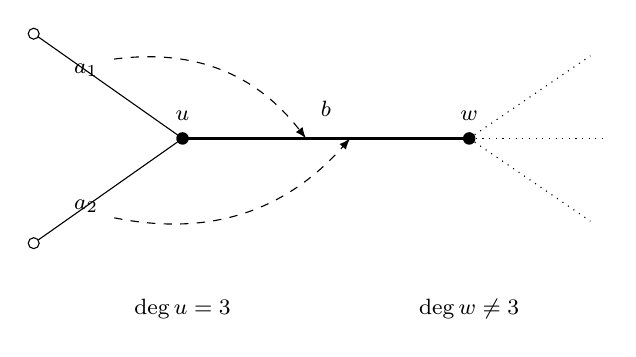
\begin{tikzpicture}[scale=1.4,>=latex]
  \coordinate (u) at (0,0);
  \coordinate (w) at (2.6,0);
  \coordinate (p) at (-1.35,0.95);
  \coordinate (q) at (-1.35,-0.95);
  \draw[very thick] (u) -- (w);
  \draw (u) -- (p) node[pos=0.52,above left=-1pt] {\footnotesize $a_1$};
  \draw (u) -- (q) node[pos=0.52,below left=-1pt] {\footnotesize $a_2$};
  \node[circle,fill=black,inner sep=1.6pt] at (u) {};
  \node[circle,fill=black,inner sep=1.6pt] at (w) {};
  \node[circle,draw=black,fill=white,inner sep=1.4pt] at (p) {};
  \node[circle,draw=black,fill=white,inner sep=1.4pt] at (q) {};
  \node[above=3pt] at (u) {\footnotesize $u$};
  \node[above=3pt] at (w) {\footnotesize $w$};
  \node at (0,-1.55) {\footnotesize $\deg u = 3$};
  \node at (2.6,-1.55) {\footnotesize $\deg w \ne 3$};
  \node at (1.3,0.27) {\footnotesize $b$};
  \draw[->,dashed] (-0.62,0.72) to[bend left=30] (1.12,0);
  \draw[->,dashed] (-0.62,-0.72) to[bend right=30] (1.52,0);
  \draw[dotted] (w) -- (3.7,0.75);
  \draw[dotted] (w) -- (3.7,-0.75);
  \draw[dotted] (w) -- (3.85,0);
\end{tikzpicture}
\caption{The worst case at a bridge $b=uw$: both other edges $a_1,a_2$ at the
degree-$3$ end $u$ are bad, and both are assigned to $b$ (dashed
arrows).}\label{fig:assign}
\end{figure}

\smallskip
\emph{Step 3: the sum.} Every other edge has $x(a) \le 0$. So
by~\eqref{eq:identity} and Table~\ref{tab:cases},
\begin{equation}\label{eq:final}
  2 \;=\; \sum_a x(a) \;\le\; \frac{P}{24} - \frac{B}{6}
     \;\le\; \frac{2B}{24} - \frac{B}{6} \;=\; -\frac{B}{12} \;<\; 0 .
\end{equation}
\end{proof}

Step~2 has room to spare: $P \le 4B$ would already give a sum of at most $0$.

\begin{remark}
Bridge-relaxed alternating plane graphs with bridges do exist. Take three copies
of the $17$-vertex $(3,4,5)$-alternating plane graph of~\cite[Figure~2]{AHSSV2015},
each drawn with a degree-$5$ vertex $z_i$ on the outer face, and join $z_1$ and
$z_3$ to $z_2$ by bridges. Then $\deg z_2 = 7$, $\deg z_1 = \deg z_3 = 6$, and
the merged outer face has size at least $13$, larger than every inner face. It
has more than two degrees and more than two face sizes.
\end{remark}

\section{What stays open}

The charge sums to a constant, so it says nothing about proportions. Alth\"ofer
et al.\ also ask how the degrees of large $(3,4,5)$-alternating plane graphs are
distributed: the ratio of degree-$4$ to degree-$3$ vertices lies in $[1,1.5]$
asymptotically, and they ask whether it has a limiting density there. A per-edge
bound cannot see that. We do not know what can.

\section*{Disclosure of AI use}

Large language models were used throughout this work. They helped search for
arguments, reviewed the proofs adversarially, and drafted the prose from the
author's notes; the author edited it. The idea of allowing bridges
(\S\ref{sec:c2}) came from an AI reviewer. The systems were Claude Opus~5 and
Claude Fable~5.1 (Anthropic), ChatGPT at its Pro tier and Codex
\texttt{gpt-5.6-terra} and \texttt{gpt-5.6-sol} (OpenAI), and DeepSeek
\texttt{v4-pro} and \texttt{v4-flash}, used from February to September 2026. The
author checked the mathematics and is responsible for it. No AI system is an
author.

\section*{Computations}

The proofs use no computation. Exact-arithmetic checks of the inequalities and
machine checks of explicit examples are archived at
\href{https://doi.org/10.5281/zenodo.22269200}{doi:10.5281/zenodo.22269200}.

\begin{thebibliography}{9}

\bibitem{AHSSV2015}
I.~Alth\"ofer, J.~K. Haugland, K.~Scherer, F.~Schneider and N.~Van Cleemput,
\emph{Alternating plane graphs}, Ars Math. Contemp. \textbf{8} (2015),
337--363.
\href{https://doi.org/10.26493/1855-3974.584.09a}{doi:10.26493/1855-3974.584.09a}.

\bibitem{BM2007}
G.~Brinkmann and B.~D. McKay, \emph{Fast generation of planar graphs},
MATCH Commun. Math. Comput. Chem. \textbf{58} (2007), 323--357.

\bibitem{CW2017}
D.~W. Cranston and D.~B. West, \emph{An introduction to the discharging method
via graph coloring}, Discrete Math. \textbf{340} (2017), 766--793.
\href{https://doi.org/10.1016/j.disc.2016.11.022}{doi:10.1016/j.disc.2016.11.022}.

\bibitem{JV2013}
S.~Jendrol' and H.-J. Voss, \emph{Light subgraphs of graphs embedded in the
plane --- a survey}, Discrete Math. \textbf{313} (2013), 406--421.
\href{https://doi.org/10.1016/j.disc.2012.11.007}{doi:10.1016/j.disc.2012.11.007}.

\bibitem{Kotzig1955}
A.~Kotzig, \emph{Contribution to the theory of Eulerian polyhedra},
Mat.-Fyz. \v{C}asopis Slovensk. Akad. Vied \textbf{5} (1955), 101--113.

\bibitem{Lebesgue1940}
H.~Lebesgue, \emph{Quelques cons\'equences simples de la formule d'Euler},
J. Math. Pures Appl. (9) \textbf{19} (1940), 27--43.

\bibitem{MT2001}
B.~Mohar and C.~Thomassen, \emph{Graphs on Surfaces}, Johns Hopkins University
Press, Baltimore, 2001.

\end{thebibliography}

\end{document}
